% Fig. M2 - Mapa de regiones operativas esperadas
% Unified style with the 8 existing figures
% Compile: pdflatex fig_m2_param_map.tex
\documentclass[border=8pt]{standalone}
\usepackage[utf8]{inputenc}
\usepackage[T1]{fontenc}
\usepackage{amsmath}
\usepackage{tikz}
\usetikzlibrary{arrows.meta, positioning, calc, patterns, fit}

\begin{document}
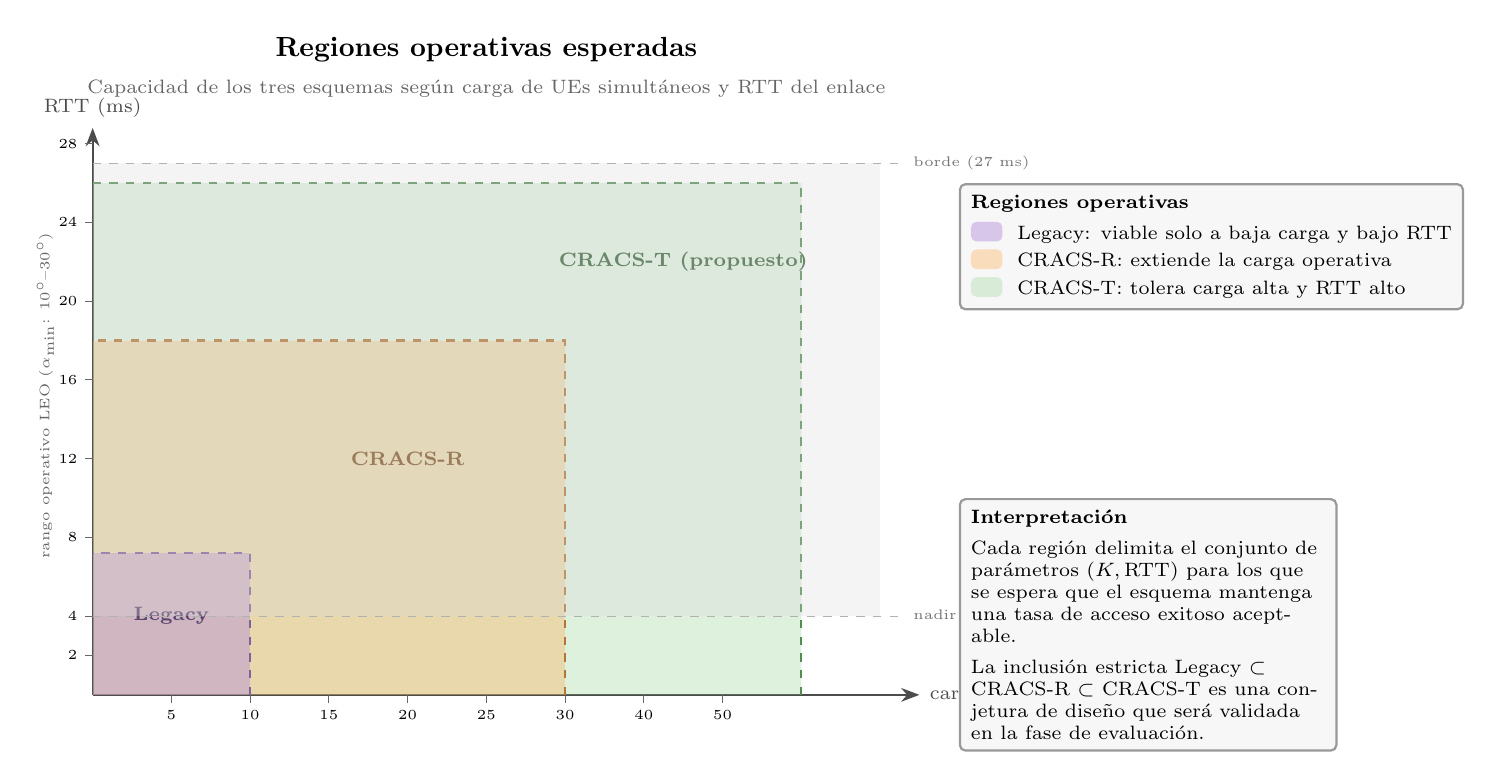
\begin{tikzpicture}[
    >=Stealth,
    font=\footnotesize,
    label/.style={font=\scriptsize, text=black!70},
    legendbox/.style={draw=black!40, fill=black!3, rounded corners=2pt,
                      inner sep=4pt, font=\scriptsize, align=left, thick=0.4pt},
]

\definecolor{regLegacy}{RGB}{180,140,220}   % purple
\definecolor{regSARA}{RGB}{255,170,80}      % orange
\definecolor{regNEW}{RGB}{120,200,120}      % green

% ============================================================
% TITLE
% ============================================================
\node[font=\normalsize\bfseries] at (5, 8.2)
    {Regiones operativas esperadas};
\node[font=\scriptsize, text=black!60] at (5, 7.7)
    {Capacidad de los tres esquemas según carga de UEs simultáneos y RTT del enlace};

% ============================================================
% AXES
% ============================================================
% X axis: number of simultaneous UEs (load)
% Y axis: RTT (ms)
\draw[thick, ->, black!70] (0, 0) -- (10.5, 0) node[right, font=\scriptsize] {carga ($K$ UEs)};
\draw[thick, ->, black!70] (0, 0) -- (0, 7.2) node[above, font=\scriptsize] {RTT (ms)};

% X axis ticks
\foreach \x/\val in {1/5, 2/10, 3/15, 4/20, 5/25, 6/30, 7/40, 8/50} {
    \draw[thin, black!60] (\x, 0) -- (\x, -0.1);
    \node[font=\tiny, below=2pt of {(\x, 0)}] {\val};
}

% Y axis ticks
\foreach \y/\val in {0.5/2, 1/4, 2/8, 3/12, 4/16, 5/20, 6/24, 7/28} {
    \draw[thin, black!60] (0, \y) -- (-0.1, \y);
    \node[font=\tiny, left=2pt of {(0, \y)}] {\val};
}

% ============================================================
% REGIONS (shaded)
% ============================================================

% Region CRACS-T (green) - largest, covers wide K and high RTT
\fill[regNEW, opacity=0.25] (0, 0) -- (9, 0) -- (9, 6.5) -- (4.5, 6.5) -- (0, 6.5) -- cycle;
\draw[thick, regNEW!70!black, dashed]
    (9, 0) -- (9, 6.5) -- (0, 6.5);

% Region CRACS-R (orange) - medium, covers moderate K and moderate RTT
\fill[regSARA, opacity=0.35] (0, 0) -- (6, 0) -- (6, 4.5) -- (0, 4.5) -- cycle;
\draw[thick, regSARA!70!black, dashed]
    (6, 0) -- (6, 4.5) -- (0, 4.5);

% Region Legacy (purple) - smallest, only low K and low RTT
\fill[regLegacy, opacity=0.45] (0, 0) -- (2, 0) -- (2, 1.8) -- (0, 1.8) -- cycle;
\draw[thick, regLegacy!70!black, dashed]
    (2, 0) -- (2, 1.8) -- (0, 1.8);

% ============================================================
% REGION LABELS (placed inside each region)
% ============================================================
\node[font=\scriptsize\bfseries, text=regLegacy!50!black]
    at (1, 1.0) {Legacy};

\node[font=\scriptsize\bfseries, text=regSARA!50!black]
    at (4, 3.0) {CRACS-R};

\node[font=\scriptsize\bfseries, text=regNEW!50!black]
    at (7.5, 5.5) {CRACS-T (propuesto)};

% ============================================================
% REFERENCE POINTS (typical operating points)
% ============================================================

% Typical LEO RTT range annotation (shaded strip)
\fill[black!15, opacity=0.3] (0, 1.0) rectangle (10, 6.75);
\node[font=\tiny, text=black!60, rotate=90] at (-0.6, 3.8)
    {rango operativo LEO ($\alpha_{\min}$: 10$^\circ$--30$^\circ$)};

% Horizontal reference lines for typical LEO RTTs
\draw[thin, black!30, dashed] (0, 1.0) -- (10.3, 1.0);
\node[font=\tiny, text=black!55, anchor=west] at (10.3, 1.0) {nadir (4 ms)};

\draw[thin, black!30, dashed] (0, 6.75) -- (10.3, 6.75);
\node[font=\tiny, text=black!55, anchor=west] at (10.3, 6.75) {borde (27 ms)};

% ============================================================
% LEGEND (bottom-right corner, compact)
% ============================================================
\node[legendbox, anchor=north west] at (11, 6.5) {
    \textbf{Regiones operativas}\\[3pt]
    \tikz[baseline=-2pt]{\fill[regLegacy, opacity=0.45]
        (0,-0.1) rectangle (0.4,0.15);}\ \ Legacy: viable solo a baja carga y bajo RTT\\[2pt]
    \tikz[baseline=-2pt]{\fill[regSARA, opacity=0.35]
        (0,-0.1) rectangle (0.4,0.15);}\ \ CRACS-R: extiende la carga operativa\\[2pt]
    \tikz[baseline=-2pt]{\fill[regNEW, opacity=0.25]
        (0,-0.1) rectangle (0.4,0.15);}\ \ CRACS-T: tolera carga alta y RTT alto
};

% Interpretation note
\node[legendbox, anchor=north west, text width=4.5cm] at (11, 2.5) {
    \textbf{Interpretación}\\[3pt]
    Cada región delimita el conjunto
    de parámetros $(K, \mathrm{RTT})$
    para los que se espera que el
    esquema mantenga una tasa
    de acceso exitoso aceptable.\\[3pt]
    La inclusión estricta
    Legacy $\subset$ CRACS-R $\subset$ CRACS-T
    es una conjetura de diseño
    que será validada en la fase
    de evaluación.
};

\end{tikzpicture}
\end{document}
